\label{app:chap3}


\section{Mesh refinement analysis}

Proper meshing is crucial in order to obtain accurate simulation data. Coarse meshes will generally result in poor results that badly represent the deformation of the system. Fine meshes will consume a lot of RAM and therefore take up a lot of computation time. Therefore, a valid mesh size needs to be obtained, which balances the accuracy of output data and computation time. To this end, multiple simulations are carried out in $\verb+Abaqus/CAE+$ to justify the mesh size.

In the simulation, both bellows are pressurized to $80$ kPa. Multiple simulations are carried out for an increased amount of nodes. These nodes are a measure for the mesh size. The elongation of the manipulator is determined for each simulation. Figure \ref{fig3:meshrefinement} shows the determined elongation as a function of the number of nodes.

\begin{figure}[H]
    \centering
    \includegraphics[width = 0.6\textwidth]{Figures/Chapter2/MeshRefinement.eps}
    \caption{Mesh refinement analysis for a bellow pressure of $80$ kPa.}
    \label{fig3:meshrefinement}
\end{figure}


Figure \ref{fig3:meshrefinement} shows that from 60 thousand nodes onwards the elongation data may be deemed reliable. A lower amount of nodes results in poor data output. Furthermore, it can be seen that increasing the number of nodes does not improve the simulation output any further. At 60 thousand nodes, the elongation has already converged.



